
\let\textcircled=\pgftextcircled
\chapter{Testing and results} \label{chap:testing}

\initial{I}n order to prove the effectiveness of the Obstacle Collision Avoidance System, it needs to be tested to check that it meets the requirements and design specifications.
Hence, a set of individual tests have to be designed to assess the capabilities of each of the components involved in the system.

The present chapter will cover the experimental setups and results of those experiments performed on the critical components, subsystems and, finally, the system as a whole in a realistic environment.


\section{Testing methods}

Most of the testing was done in parallel to the implementation of the design into the real product, ensuring that the system was built over robust and properly working components, since possible modifications to the design are significantly more costly the later the development phase in which errors are detected (see Figure \ref{fig:incose}).
Furthermore, tests can give valuable insight on the functioning of the components, which can prove useful in the decision making process within the implementation stages, effectively improving the overall performance of the system.

Thus, the actions described in this chapter can be seen as complementary and, in some sense also contributing, to the implementation phase of the OCAS.

\subsection{Component testing}

The validation of each individual component is assumed to be successfully done by the manufacturer.
Therefore, comprehensive testing will only be performed on the parts of the system that have been actively developed during the execution of this project, such as the interfaces and the operation algorithms of the ultrasonic rangefinders, since they are a critical component of the OCAS.

\subsubsection{Interfaces}

Assuming that the stock UAV interfaces (RC transmitter / receiver, telemetry link with GCS) are already tested and working, the connections to be verified are those involving the OCAS only, shown in Figure \ref{fig:ocas}.
In particular, the GCS connection over WiFi is of higher interest, since the power connection is straightforward to check by ensuring that the Raspberry Pi boots when plugged; and the MAVlink serial connection should not entail any difficulty once the appropriate communication port and baud rate are selected upon startup of MAVproxy (which is automatically done when using the GUI for that purpose).
Also, the testing of the GPIO connection will be covered in Section \ref{sec:sonartest}.

Concerning the network connection of the Raspberry Pi, it is controlled by the Raspbian OS.
Having set up the ad-hoc network from the Windows machine at the GCS as specified in Appendix \ref{app:network}, the Dynamic Host Configuration Protocol (DHCP) server should be properly configured to imitate the Local Area Network (LAN) settings to which the GCS machine is connected.
Thus, the DHCP service will provide the Raspberry Pi with a compatible IP, together with other important network parameters, automatically. 

Nevertheless, the problem with DHCP is that the address of the computers connected to the network will occasionally change, altering the settings for a successful SSH connection (those varying settings can be found by following the steps in Appendix \ref{app:ssh}).
Thus, for a more convenient debugging option, an static IP interface was selected on the Raspberry Pi's ethernet port.

Finally, in order to resemble the described setting on the Raspberry Pi, the configuration must be done by modifying the \texttt{interfaces} file which is present in all Debian-based Operating Systems at /etc/network/interfaces.
The specific file for the OCAS computer board is copied in Appendix \ref{app:interfaces} for completeness, together with an example of the \texttt{wpa\_suplicant.conf} file which holds the parameters for the wireless network connections.

In terms of the evaluation of the connection, considering the scope of the project, it is considered that the interface is successfully connected if the communication is responsive and stable, which can be certainly proven by construction\footnote{From Wolfram Mathworld: A constructive proof is a proof that directly provides a specific example, or which gives an algorithm for producing an example. Constructive proofs are also called demonstrative proofs}, following the steps in Appendices \ref{app:network} and \ref{app:ssh}.

\subsubsection{Ultrasonic rangefinders} \label{sec:sonartest}

The selected HC-SR04 sensors are mainly built to be connected to Arduino microcontrolers, which operate at 5 V.
Hence, in order to obtain some familiarity with their usage, as documented by the manufacturer (see Appendix \ref{app:sonar-doc}), the operation was initially made from an Arduino Mega board, which would trigger the ultrasonic signal and receive the processed echo to be transformed into the distance to the closest obstacle.

Ensuring that all the connections on the Arduino board were successful, the following logical step is to perform the same test from the Raspberry Pi, which inherits the inclusion of the voltage dividers (Figure \ref{fig:voltage}) and the Python GPIO libraries.
It was during this stage that the \texttt{Sonar} class was developed, requiring only a ``driver'' file that would make calls to the \texttt{Sonar}'s methods, which can be found in Appendix \ref{app:sonarDriver}.

Apart from triggering the ultrasonic rangefinders, the driver file would print the measured distance for any amount of attached sensors and display a graph with their values together with the calculated velocity, to help with their study in the Results section.

On the hardware side, it is known that the ultrasonic rangefinders are rather directional sensors and do not perform at their best if the obstacle is not situated directly on the symmetry plane.
In order to assess the maximum spatial capability of the sensors, a 4m$^2$ aluminium plate was used as object to be detected, placing it in various positions in order to determine the spatial range limits in terms of maximum angles at which the ultrasonic signal is adequately reflected back to the sensor, getting a successful reading on the distance.


\subsection{Software testing: SITL}

Prior to the implementation of the OCAS in the real UAV, and knowing by individual tests that the hardware components were working properly, it was necessary to test the definition of the MAVlink messages that were to be sent to control the UAV in flight.
Furthermore, it was of utmost importance that the navigation coordinates were correctly defined, and also the transformations between different reference systems, since the MAVlink protocol only supports commands in the global (latitude, longitude, altitude) reference system, while for physical obstacle navigation it is more convenient to define the procedures either in Flat Earth (North, East, Down) or even body fixed (x, y, z) reference frames, from which the transformations needed to be computed.

To ensure safety during the software testing phase, the scripts were initially tested in a simulator.
In particular, the DroneKit development team provides a Software-In-The-Loop (SITL) simulator that works in a similar manner than a real Ardupilot UAV would.

Software-In-The-Loop means that, for the control algorithms, only software input is considered.
Hence, the physical characteristics of the UAV, together with its default sensors (IMU, barometer, GPS\ldots) all have what is considered to be a reasonably accurate software representation of their hardware counterparts (accuracy which, in the case of the SITL simulator, is not where the emphasis has been put as studied in \cite{vegaastorga2016}).
Nevertheless, the existent inaccuracies do not present any major problems for the script testing since the closed-loop PID control algorithms ensure that disturbances and errors are cancelled, finally reaching the requested state albeit by taking slightly different transient responses.

What is of higher importance in the software testing phase is the actual interpretation of the MAVlink commands by the Ardupilot control board, and the general physical response to them.
Fortunately, it is in the Ardupilot firmware simulation where the SITL software excels, since the simulator runs the exact same source code, only adapted to run on a regular computer rather than an Arduino board and to receive input from the software models rather than the real sensors.

However, the simulation of the default sensors via software means that the OCAS is not implemented (for being a custom build for this project).
Thus, the $t_{safe}<0$ condition can not be computed in the simulated environment.
For the purpose of testing, the sonars step in the \texttt{main.py} file of the custom script was adapted to include the monitorisation of Channel 7 on the RC transmitter, which would cause the same reaction as the ultrasonic rangefinders at the change of state of the corresponding switch, by modifying the lines 41 to 93 on Appendix \ref{app:main} by the fragment of code in Appendix \ref{app:ch7}, accompanied by the \texttt{Observe} class from Appendix \ref{app:observe}.

Finally, it is worth mentioning the role of the simulator within the rest of the subsystems of the OCAS, since SITL is only aimed at replacing the UAV block from Figure \ref{fig:ocas}.
The MAVlink stream of data out of the simulator is transmitted using the TCP protocol, which can be substituted in the MAVproxy startup options instead of the serial address that is used for the connection with the UAV.
Hence, the two leftmost blocks in Figure \ref{fig:mavproxy} would be substituted by the simulator, with the TCP interface with MAVproxy, being this change completely transparent to the Python script, which does not need any further modification.

In addition, in the Windows version of the GUI application, the option to launch the simulator and autocomplete the address and port fields on the MAVproxy parameters (see Figure \ref{fig:gui}) was included to facilitate the testing stages of the project, together with the Mission Planner button, which greatly simplify the testing workflow.

\subsection{System testing}


\begin{wrapfigure}{r}{0.5\textwidth}
	\centering
	\vspace{-1em}
	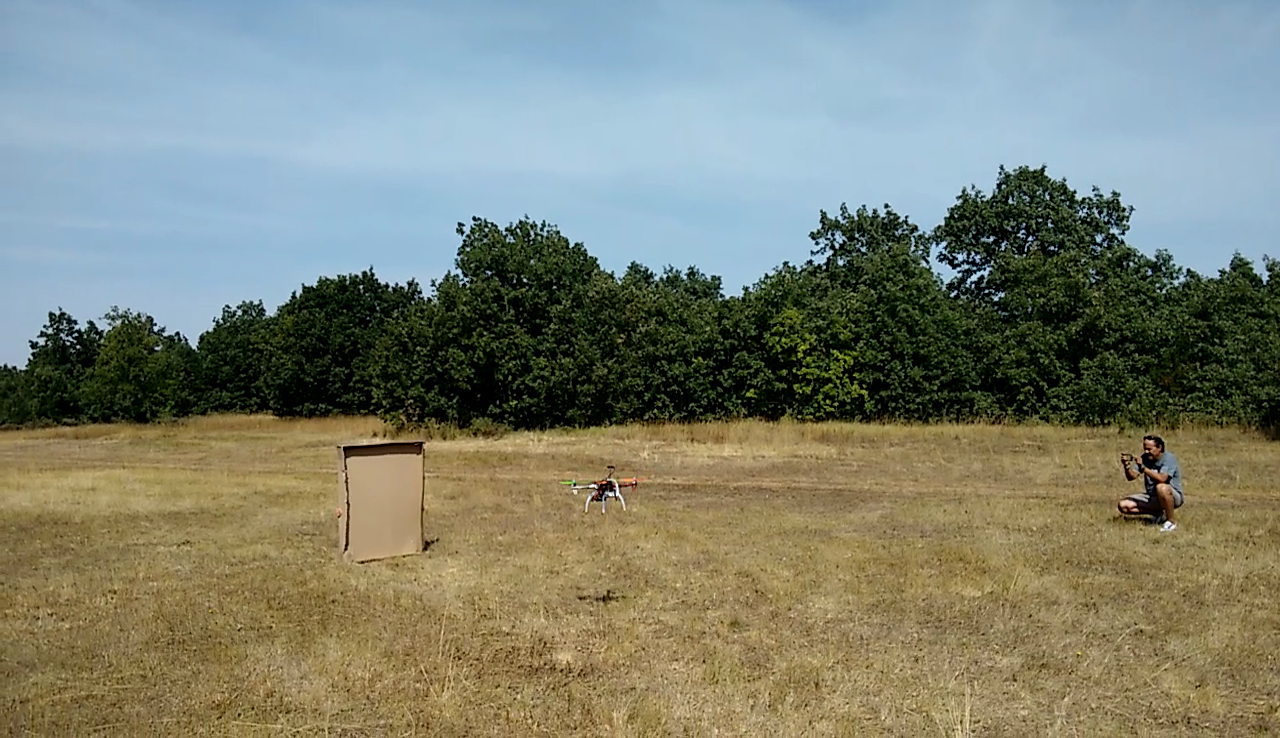
\includegraphics[width=0.5\textwidth,clip,trim={6cm 2cm 17cm 9cm}]{./figures/obstacle.png}
	\caption{Testing obstacle}
	\label{fig:obstacle}
\end{wrapfigure}


As the last step in the validation process, the OCAS shall be tested as a complete system in a realistic scenario.
For that purpose, the full operative UAS was taken to a flight field and flown against a simulated soft (cardboard) obstacle to avoid any serious damage in case of failure, as shown in Figure \ref{fig:obstacle}.
In this stage, the logs (defined in Section \ref{sec:logging}) acquire maximum importance since they allow to compare and contrast the data and sequence of events with the video footage from the tests.


\section{Results}

In the present section, the results concerning the previously described tests from which a valuable lesson can be extracted will be discussed.
Successful tests in which the systems work as expected will be left out of the discussion in the case that they do not contribute to any further knowledge on the functioning of the system.

\subsection{Ultrasonic rangefinders}

Two main issues appeared when assessing the performance of the sonars: First, the Field Of View (FOV) of each individual sensor is quite limited, which encouraged for the incorporation of an array of several sensor with slightly different orientations to cover a wider range.
On the other hand, the implementation of more than one rangefinder created some unwanted effects when operating simultaneously, since the signal from one of them could be seen as the echo reflection of the previously triggered sensor, causing ghost signals and bad readings.

In terms of the sonar's capabilities, the tests with the aluminium plate as obstacle placed at approximately 2 m from the sensor unveiled that their maximum FOV against a large surface completely perpendicular to the line of sight is of 35$^\circ$, while the maximum inclination that reflects a valid signal is of 20$^\circ$ with respect to the plane of symmetry, as shown in Figure \ref{fig:plate}.

\begin{figure}[htbp]
	\centering

	\begin{tikzpicture}

		\begin{scope}[rotate=-35,local bounding box=plate1]
				\path[shade,bottom color=white,top color=black!70] (1.5,6.5-1) arc[radius=1,start angle=270,end angle=305] -- (1.5,6.5) -- cycle;
				\node[inner sep=0] at (1.5+0.35,6.5-1.2) {\footnotesize < 35$^\circ$};
			\draw[thick] (0,0) -- (3,0);
			\foreach \c in {0,1,2,...,20}
				\draw (\c/7,0) -- ($(\c/7,0)+(0.2,-0.2)$);
			\draw[dashed] (1.5,0) -- (1.5,6.5);
			\draw (1.5-0.2,0) arc[radius=0.2,start angle=180,end angle=90];
			\draw[fill] (1.5-0.08,0.08) circle[radius=0.15mm];
		\end{scope}

		\begin{scope}[rotate=20,shift={($(plate1.center)+(-0.28cm,-3.9cm)$)}]
				\path[shade,left color=white,right color=black!70] (1.5-1,0) arc[radius=1,start angle=180,end angle=160] -- (1.5,0) -- cycle;
				\node at (0.5,0.2) {\footnotesize < 20$^\circ$};
			\draw[thick] (0,0) -- (3,0);
			\foreach \c in {0,1,2,...,20}
				\draw (\c/7,0) -- ($(\c/7,0)+(0.2,-0.2)$);
			\draw[dashed] (1.5,0) -- (1.5+6.5*sin{20},6.5*cos{20});
			\draw[thin,dashdotted] (1.5,0) -- (1.5-1*cos{20},1*sin{20});
		\end{scope}

		% Sonar
		\coordinate(coord) at (1.5*cos{35}+6.5*sin{35},-1.5*sin{35}+6.5*cos{35});
		\path[fill=blue!70!black!80] ($(coord)+(-1,0)$) rectangle ($(coord)+(1,0.05)$);
		\path[draw,fill=gray!70] ($(coord)+(-0.8,0)$) rectangle ($(coord)+(-0.3,-0.3)$);
		\path[draw,fill=gray!70] ($(coord)+(0.8,0)$) rectangle ($(coord)+(0.3,-0.3)$);
		\node[above=0.1cm of coord]{Sonar};

		\node[below=3cm of coord,xshift=0.5cm]{$\approx$2m};

		\begin{scope}

		\end{scope}

	\end{tikzpicture}

	\caption{Ultrasonic rangefinder FOV test setup}
	\label{fig:plate}
\end{figure}


These limitations in the maximum FOV imply that more than one sensor with slightly different orientations shall be used to cover the complete space in front of the UAV.
For the first prototype, 3 sonars were mounted with approximately 20$^\circ$ between them, which ensures that the complete frontal path is covered during forward flight.

However, operating more than one ultrasonic rangefinder generates an additional problem, since they generate and receive identical signals for their measurements, implying that the signal generated from one sensor can be captured by a different one, creating misleading signal flight times.
This problem can be mitigated in two different ways.
First, triggering the sonars all at the same time would generate an assortment of similar signals from which no sensible discrimination can be done; the solution is to send the trigger signals at different intervals in time, ensuring that the echo signal from one sonar is received before the trigger signal of the next one is sent.
Nevertheless, there can still be lost signals and multipath errors which need to be alleviated.
Thus, the second step can be to filter the signals to account for suspicious discrepancies, which in the scope of the first prototype was done by performing the rolling average of the last several measurements (see Section \ref{sec:measureDistance}), although more advanced signal processing techniques can definitely provide better results.


\subsection{Simulator} \label{sec:sitl}

There is one essential difference between a simulator and reality: any simulator represents a model of the physical world, but the physical world is so complex that no simulator can achieve an infinitely precise representation of reality.

That being said, there are some physical effects that are not implemented in the SITL simulator. For example, the input from the simulated sensors perfectly represents the calculated state of the UAV, albeit with some artificial gaussian noise added to them according to their individual accuracy and response rates.

This fact became a problem when the SITL validated software was to be tested on the real UAV.
For example, while the relative location computations and MAVlink commands appeared to work perfectly well in the simulator, there was some unknown phenomenon that was causing the real UAV to behave violently instead of maintaining the position when the Guided mode was activated by the script.

After several weeks trying to find the root of the problem, and analysing all the inputs that could be affecting the behaviour of the Ardupilot controller, it was concluded that, since the GPS sensor was a requirement for the loitering capabilities of the Guided mode, and the tests were being done in a controlled space within the city (see Figure \ref{fig:leganes}), surrounded by high buildings, there was a significant chance that the reception of the very weak GPS signals from the satellites (orbiting in Medium Earth Orbit at around 20,200 km) were being blocked and / or affected by the surrounding walls.

\begin{figure}[htbp]
	\centering
	\begin{tikzpicture}
		\node[opacity=0.7]{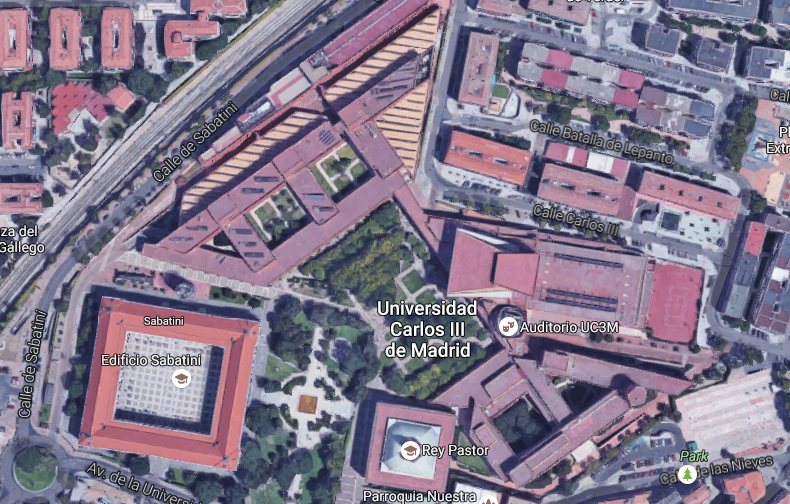
\includegraphics[width=0.8\textwidth]{./figures/leganes.png}};
		\node[rectangle,draw=red,line width=1mm,rotate=35,shift={(0.05cm,1.6cm)},minimum width=1cm,minimum height=1cm]{};
	\end{tikzpicture}
	\caption{Initial testing site within the city}
	\label{fig:leganes}
\end{figure}


This phenomenon is called multipath error: the GPS sensor can determine its position by receiving the signals from at least 4 satellites for which their location in the sky (ephemeris) and the precise time of transmission of those messages is known.
By comparing the time of arrival of the signal with the time of emission, the GPS module can calculate the exact distance to that particular satellite.
Then, by triangulating (intersecting the spherical loci of) those distances (and solving for the clock bias), the global position of the vehicle can be precisely determined.
However, the high propagation speed of the electromagnetic waves (speed of light, $\approx 3\times 10^8$ m/s) conveys that a small mismatch in the time of arrival of the signal can generate large errors in the final calculated distance from the GPS module to the satellite.
Furthermore, the GPS signals can rebound on the walls of buildings, effectively covering more distance than the straight line that joins the satellite and the sensor, significantly magnifying the effect.

Once the possible source of error was pointed down, the only action needed to verify or discard it was to move to a countryside location for the tests, which indeed proved the multipath error to be the source of the unwanted behaviour of the UAV in the preceeding tests.

The lesson to be learnt from these events is the dependence of the Guided mode on a high quality GPS signal, which implies that the solution presented in this thesis is not still applicable to indoor nor urban flight; at least not if the control commands encode information on the global location of the UAV.
Nevertheless, in future work, some control procedures could be implemented in order to consider the input streams from the ultrasonic rangefinder as the main source of information for the navigation algorithms, overriding the RC transmitter channels directly instead of commanding higher level ``go-to'' manoeuvres to the Ardupilot control board.

\subsection{UAS + OCAS}

Finally, it is necessary to confirm that each of the subsystems are properly integrated and are able to work together for a common goal within the UAS.
After a realistic test flight, the logged information provides some valuable insight on the execution of the tasks and their effectiveness to actually avoid the collision with foreign obstacles.

For the selected flight test, vast amounts of data are recorded (more than 5000 individual messages) containing information on the complete state of the UAV as recorded from all the onboard sensors.
Fortunately, since the particular script that was run defined as the avoidance manoeuvre to command a climb of the vehicle and the vehicle was flying mostly forward during the test, the different stages of the flight can be easily recognised from the relative altitude and the y-position with respect to the take off location in the body-fixed reference frame plots, depicted in Figures \ref{fig:h_flight} and \ref{fig:y_flight}, respectively.

Additionally to Ardupilot's logs, the data recorded from the Python script itself is overlayed to show the precise moments at which commands are being sent to the UAV, and its response to them, indicating who is in control of the vehicle as the test progresses.
Furthermore, from the telemetry logs the flight modes of the UAV at any instant of time can be extracted, as are displayed at the bottom of the plot.


\begin{figure}[htbp]
	\centering
	\begin{subfigure}{\textwidth}
		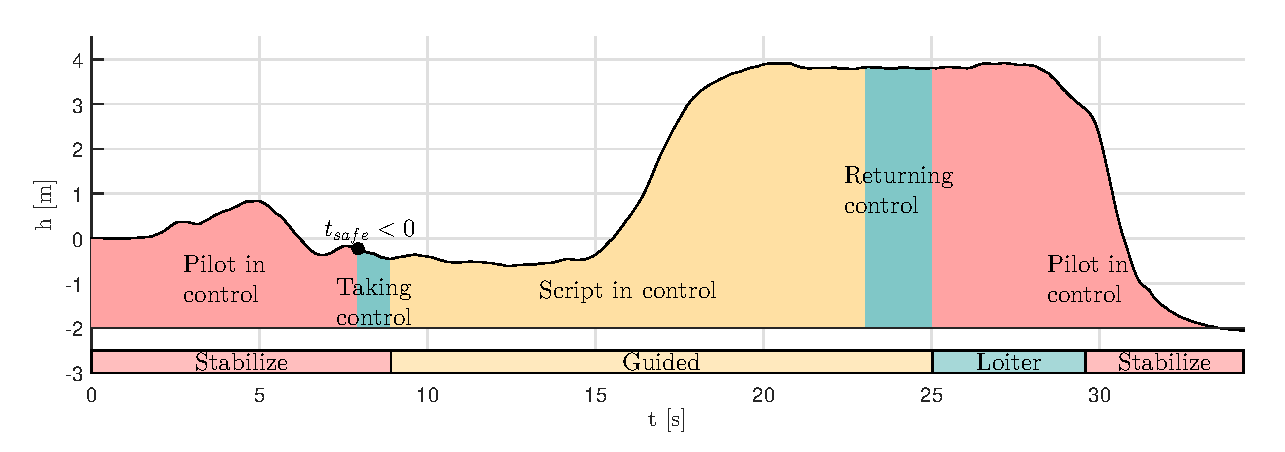
\includegraphics[width=\textwidth]{./figures/h_flight.eps}
		\caption{Relative altitude during the flight test}
		\label{fig:h_flight}
	\end{subfigure}
	\begin{subfigure}{\textwidth}
		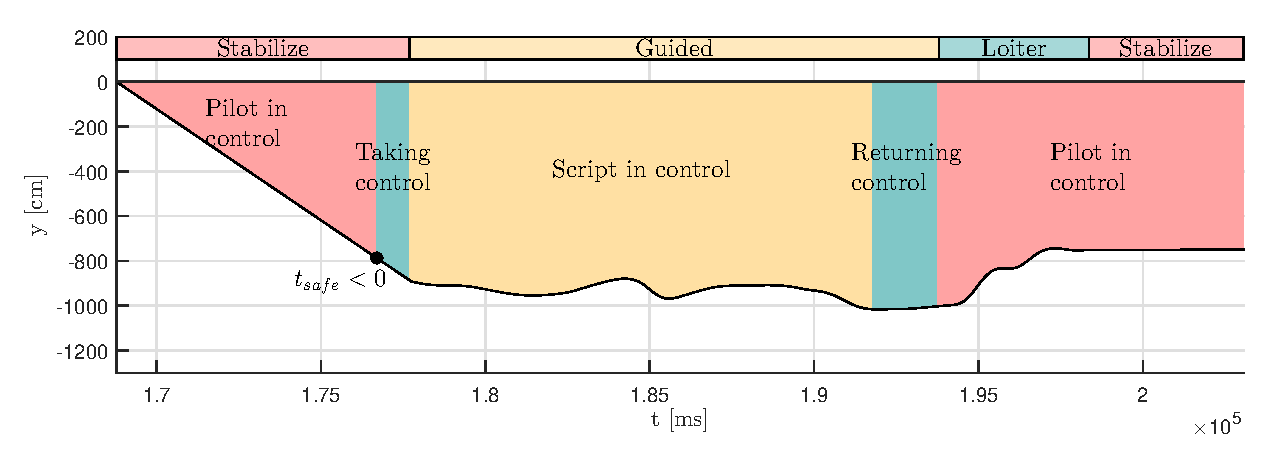
\includegraphics[width=\textwidth]{./figures/y_flight.eps}
		\caption{Longitudinal position during the flight test}
		\label{fig:y_flight}
	\end{subfigure}
	\caption{Results of the flight test}
	\label{fig:flight}
\end{figure}


As it can be seen, the initial stages of the flight are quite unsteady on the altitude side while the pilot tries to approach the testing obstacle.
Then, when the ultrasonic rangefinders determine that the state of the UAV with respect to the obstacle is not safe enough, the Guided mode gets activated (after a $\approx$1 second delay), and the vehicle stabilises trying to keep the position of activation of the mode and effectively stopping the UAV while the command is sent.
A set of functions translates the position that lies exactly 4 metres over the actual position of the UAV at the time of the computation and sends the MAVlink message to Ardupilot, which starts to climb to the commanded location, which will be maintained until the pilot is given back control.
Notice that the GPS localisation is only accurate up to one metre, and small variations can be seen on the horizontal position of the UAV for that reason, while the altitude is better maintained during the Guided phase as a result of the more precise barometer.

After a small delay, the Python script assumes that the UAV has reached the commanded location, and proceeds to return control to the pilot, which takes $\approx$2 seconds.
The control of the vehicle is given back to the pilot in Loiter mode, since it allows for adjustments in the horizontal plane while the vertical controls behave similarly to Altitude Hold mode (see Chapter \ref{chap:ardupilot}), allowing for a smooth transition.
Finally, the pilot changes back to Stabilize mode and performs the landing manually.
Observe that the landing altitude lies 2 metres below the reference take off altitude; such discrepancy is due to the fact that the take off was done from an elevated site to avoid false-positive activation of the avoidance stage by the reflection of the ultrasonic signals on the ground itself.

